%\documentclass[a4paper, 12pt]{scrreprt}

\documentclass[a4paper, 12pt]{scrartcl}
%usepackage[german]{babel}
\usepackage{microtype}
%\usepackage{amsmath}
%usepackage{color}
\usepackage[utf8]{inputenc}
\usepackage[T1]{fontenc}
\usepackage{wrapfig}
\usepackage{lipsum}% Dummy-Text
\usepackage{multicol}
\usepackage{alltt}
%%%%%%%%%%%%bis hierhin alle nötigen userpackage
\usepackage{tabularx}
\usepackage[utf8]{inputenc}
\usepackage{amsmath}
\usepackage{amsfonts}
\usepackage{amssymb}

%\usepackage{wrapfig}
\usepackage[ngerman]{babel}
\usepackage[left=25mm,top=25mm,right=25mm,bottom=25mm]{geometry}
%\usepackage{floatrow}
\setlength{\parindent}{0em}
\usepackage[font=footnotesize,labelfont=bf]{caption}
\numberwithin{figure}{section}
\numberwithin{table}{section}
\usepackage{subcaption}
\usepackage{float}
\usepackage{url}
%\usepackage{fancyhdr}
\usepackage{array}
\usepackage{geometry}
%\usepackage[nottoc,numbib]{tocbibind}
\usepackage[pdfpagelabels=true]{hyperref}
\usepackage[font=footnotesize,labelfont=bf]{caption}
\usepackage[T1]{fontenc}
\usepackage {palatino}
%\usepackage[numbers,super]{natbib}
%\usepackage{textcomp}
\usepackage[version=4]{mhchem}
\usepackage{subcaption}
\captionsetup{format=plain}
\usepackage[nomessages]{fp}
\usepackage{siunitx}
\sisetup{exponent-product = \cdot, output-product = \cdot}
\usepackage{hyperref}
\usepackage{longtable}
\newcolumntype{L}[1]{>{\raggedright\arraybackslash}p{#1}} % linksbündig mit Breitenangabe
\newcolumntype{C}[1]{>{\centering\arraybackslash}p{#1}} % zentriert mit Breitenangabe
\newcolumntype{R}[1]{>{\raggedleft\arraybackslash}p{#1}} % rechtsbündig mit Breitenangabe
\usepackage{booktabs}
\renewcommand*{\doublerulesep}{1ex}
\usepackage{graphicx}
\usepackage{chemformula}



\begin{document}

\section {Auswertung}
Um eine Relation zwischen Leitfähigkeit und Konzentration des Produktes zu erhalten, wurde eine Eichgerade durch die lineare Regression der Kalibrierungsmessreihe bestimmt (vgl. Abbildung \ref{Eichgerade}). Ferner wurde die Konzentration der Urease im Prozess als Konstant angenommen ($ 78\,[\si{\mu S}]$) und von jeder Messung subtrahiert, um aus der vorliegenden Leitfähigkeit die Produktkonzentration gemäß folgender Gleichung abzuleiten : \\
\\
Sei : \\
 $c[P]_M$ die Konzentration des Produktes in einer Messung\\
 $\sigma_M$ die gemessene Leitfähigkeit\\
  $\sigma_U$ die konstante Leitfähigkeit der Urease bei gegebener Verdünnung \\
  $f()$ die Eichfunktion, die eine Leitfähigkeit in die Produktkonzentration abbildet.\\
  \\
  Es gilt :
\begin{equation}
c[P]  \sim f(\sigma_M-\sigma_U)
\label{Eichgleichung}
\end{equation}
\begin{figure}[H]
	\centering	
	\begin{minipage}{1\textwidth}
		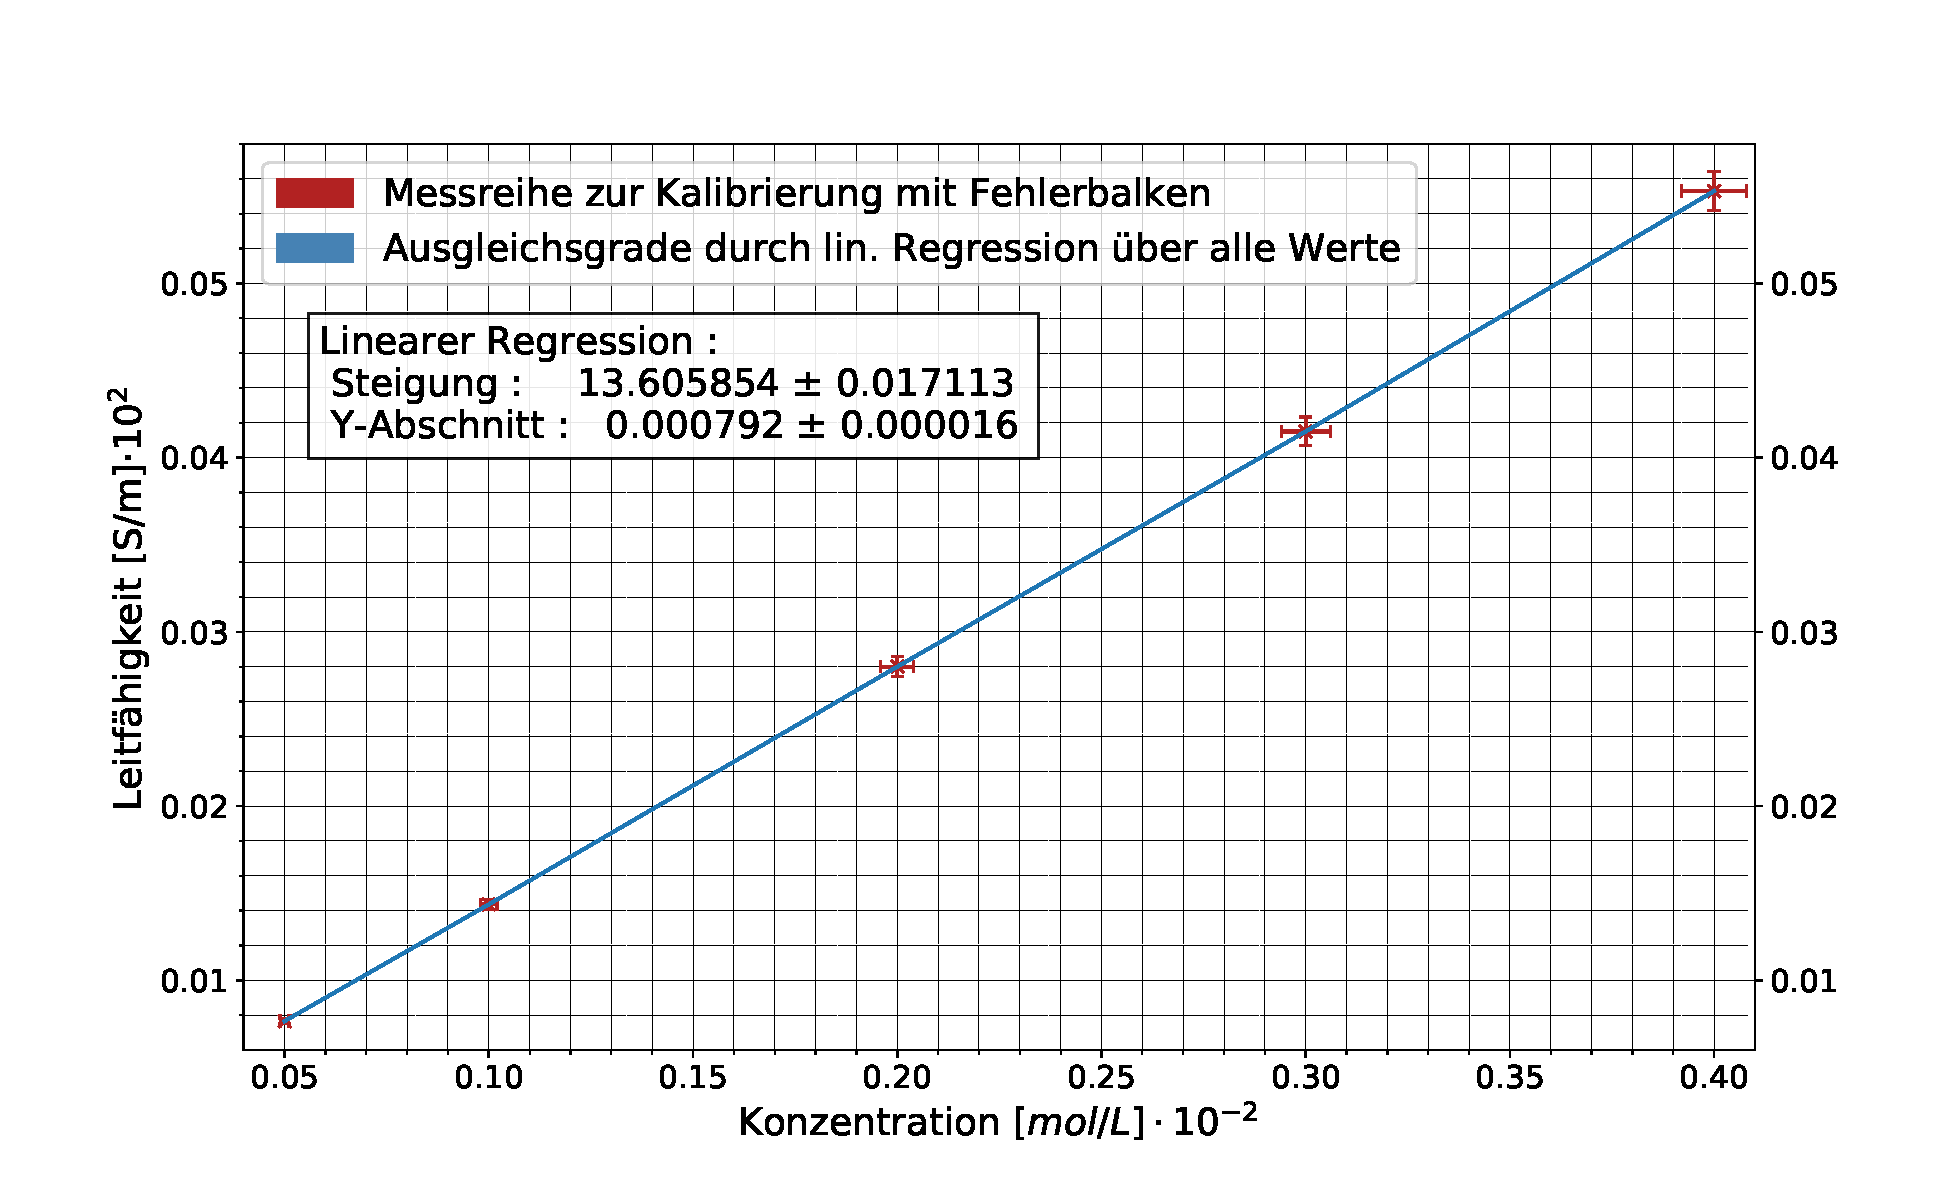
\includegraphics[width=\columnwidth]{\Bilder\Kalibierung.pdf}
	\end{minipage}
	\caption{Eichgerade mithilfe der lineare Regression der Kalibrierungsreihe durch eine Routine in der Programmiersprache \textit{python}. Fehlerbalken resultieren aus Messungenauigkeit sowie Abmessungsfehler sowie dem Fehler des Verfahrens.}
	\label{Eichgerade}
\end{figure}
Im folgenden Schritt wurden die neun durchgeführten Messreihen in einer Abbildung als zeitliche Messung der Konzentration aufgetragen. Insbesondere wurde hierfür Gleichung \ref{Eichgleichung} verwendet um aus der eigentlich gemessene Leitfähigkeit die Konzentration zu bestimmen. Der Fehler ergibt sich hier als Fehler des Verfahrens sowie als Fehler basierend auf der fehlerbehaftete Eichfunktion.
\newpage
\begin{figure}[H]
	\centering	
	\begin{minipage}{1\textwidth}
		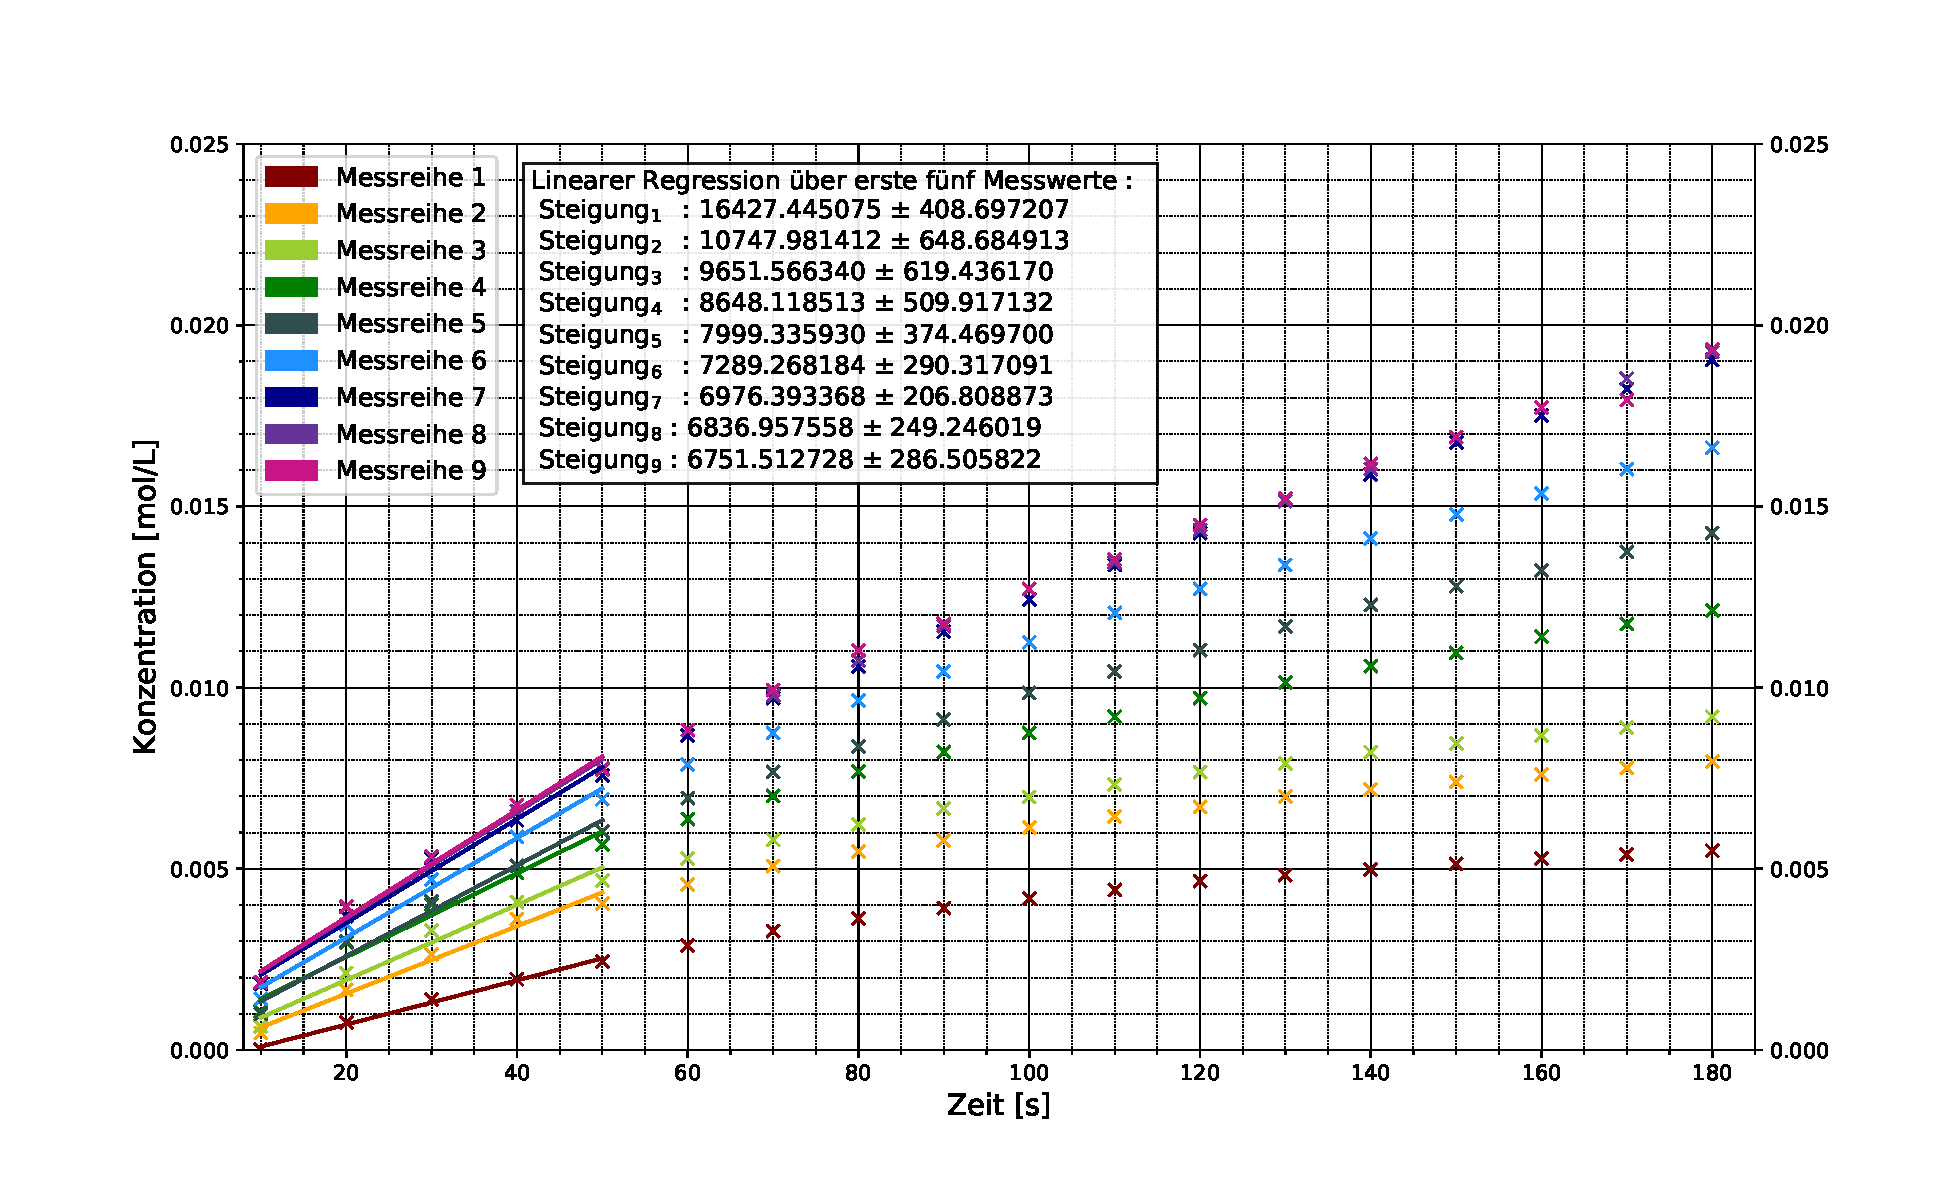
\includegraphics[width=\columnwidth]{\Bilder\Messreihe.pdf}
	\end{minipage}
	\caption{Auftragung der neun durchgeführte Messreihen der Konzentration über der Zeit. Die Ausgleichsgeraden im Bereich der ersten fünf Messpunkte wurde durch eine lineare Regression in der Programmiersprache \textit{python} erzeugt, ferner die Steigung dieser Geraden ermittelt sowie dessen Fehler.}
	\label{Messreihe}
\end{figure}
Die erhaltenen Steigungen bezogen auf die verwendete Verdünnung sowie der zugehörigen Fehler wurden in folgender Tabelle in signifikanten Stellen angegeben.
\begin{table}[H]
\centering
\label{Steigungstabelle}
	\caption{Steigungen der Ausgleichsgraden, welche durch eine lineare Regression der ersten fünf Messwerte erhalten wurden. Die lineare Regression erfolte über eine Routine in \textit{python}}
	\begin{tabular}{C{0.15\linewidth}|C{0.1\linewidth}C{0.25\linewidth}C{0.3\linewidth}}
		Messreihe $\in \mathbb{N}$ &  Steigung ($m$) &  Absoluter Fehler ($\Delta m$) & Konzentration Harnstoff $\si{[mol/L]}$ \\
		\hline \addlinespace[1ex] 
		$ 1$ & 675 & $\pm 29$ & 0.005\\
		$2$ & 683& $ \pm 25$ &0.010\\
		$3$ & 698& $\pm 21$ &0.015\\
		$4$ &729& $\pm 30$&0.02\\
		$5$&  800&  $\pm 37$ &0.03\\
		$6$&  864&  $\pm 51$&0.04\\
		$7$ &  966&$\pm 62$&0.06\\
		$8$ & 1075&$\pm  65$ &0.08\\
		$9$ &  1643& $\pm 41$ &0.1\\
	\end{tabular}
\end{table}
Mithilfe dieser wurde ein \textit{Lineweaver-Burk-Plot} angefertigt um die gesuchten Größen $v_{max}\, , \, K_M\, ,\, k_2$ aus den bestimmten Steigungen, also Anfangsgeschwindigkeiten $v_0$, zu bestimmen. Hierfür wurde insbesondere Gleichung xyz verwendet, sowie die Annahme eines linearen Verlaufs (Reaktionsordnung Null) für die ersten Messwerte.



\end{document}